%% This is an example first chapter.  You should put chapter/appendix that you
%% write into a separate file, and add a line \include{yourfilename} to
%% main.tex, where `yourfilename.tex' is the name of the chapter/appendix file.
%% You can process specific files by typing their names in at the 
%% \files=
%% prompt when you run the file main.tex through LaTeX.
\chapter{Evaluation}
\label{chap:eval}
All evaluation was done on a Mid 2012 15 inch MacBook Pro with 2.7 Ghz Intel Core i7 processor and 16GB of RAM, equipped with a solid state drive (SSD). All VMs were running on the same host, though VM2Docker makes no such restriction in practice, as only the IP address of each VM is required. The practical convenience of running on the same host allowed for a drastic speed improvement when transferring the entire VM's filesystem over the socket from agent to chief, as opposed to over a potentially slower network connection.

In section~\ref{sec:evalstrat} we outline our strategy for evaluating the different aspects of VM2Docker, and in sections~\ref{sec:evalquant} and~\ref{sec:evalqual} we discuss the results of these quantitative and qualitative measures, respectively.

\section{Evaluation Strategy}
\label{sec:evalstrat}
When attempting to evaluate the performance and effectiveness of the VM2Docker framework, we must first describe the variables of interest and the overall benefits of the Docker container format. The most explicit benefits, as introduced in chapter~\ref{chap:docker}, are those related to the performance benefits, as well as portability, of the Docker format. Since Docker containers are more lightweight than their VM counterparts, containers are much quicker to startup and have generally less performance overhead and are more comparable to running directly "native" on the host. As a result of this improved performance, hosts can also support a higher density of running containers as compared to the corresponding virtual machines.These benefits are universal to the Docker framework and are not in any way affected by the specifics of the VM2Docker framework. Therefore, we acknowledge that these benefits are essential and must be considered when deciding whether to use virtual machines or Docker containers, but that they will not be directly quantified when evaluating the effectiveness and performance of the VM2Docker system as a whole.

One of the other major benefits of the Docker framework is a consequence of its unique, layered filesystem. When containers are built, stored, and deployed, the Docker Engine makes aggressive use of caching of previous layers in order to improve build and deployment time. For example, if a Dockerfile used to generate a Docker image has already been built and is then modified by the addition of one more command at the end of the file, the Docker Engine will not need to rebuild the entire Docker image from scratch. Instead, it will automatically recognize that all layers up to the last one have already been built (and cached), and it can quickly generate a new image just by layering one command on top of the already existing Docker image. In addition to build time, deployment time and storage space can also be greatly improved by the automatic layering provided by VM2Docker. As mentioned in section~\ref{sec:dockerimport}, without VM2Docker, the only automatic method of converting a VM to the Docker format is one huge layer, in its entirety, using the Docker import tool. Every time this container is deployed, the contents of the entire filesystem must be transmitted over the network from the Docker registry to the host wishing to run the container. This gets especially wasteful when multiple containers, imported from VMs, need to be deployed. Even if they are identical except for perhaps a few packages or other files that have been changed, the entire VM must be transmitted over the network to be deployed, and the additional Docker image takes up an identical additional amount of space as the original VM. 

As the number of layers and the sharing of these layers increase across multiple VMs, Docker has the ability to improve deployment time, by transmitting only the necessary layers, and overall space usage. This is the primary quantitative metric by which we evaluate the VM2Docker system across multiple releases of three different operating systems: Ubuntu, CentOS, and Mageia. We first focus on the conversion of a single VM and analyze the relative size of each layer in the resulting Docker image, with and without package detection. We look at the results of using the two aforementioned diff strategies (\texttt{rsync} and \texttt{rdiffdir}). Then, we expand the set of inputs to multiple virtual machines at a time, with varying amounts of filesystem contents in common across many different layers in order to analyze the space savings as a function of $N$, the number of virtual machines.

Additionally, we briefly discuss the benefits of minimizing the complexity of each Dockerfile as a function of the number of packages included for a given install instruction. As mentioned in section~\ref{sec:depdetection}, we present the results of the application of dependency detection on minimizing the length of a given package install list without affecting the resulting built Docker image.

We also spend some time qualitatively describing the process of making use of VM2Docker for these three distinct operating systems and their respective package management tools.

Finally, although we focus on the filesystem layer sizes that VM2Docker produces, we also briefly mention the time required to successfully convert and deploy a set of VMs to their Docker counterparts. These absolute numbers are less essential because the conversion must only proceed once. However, we still spend some time describing certain factors that may affect the conversion time, such as network throughput, hard drive speed, and the number of packages installed.



\section{Quantitative Results}
\label{sec:evalquant}
In the following section, we evaluate the quantitative results of the VM2Docker framework. Primarily, we focus on disk usage and the relative sizes of various different layers that VM2Docker creates. Next, we touch on the ability for VM2Docker to make use of dependency detection to cull the list of packages required to recover the original VM, in its entirety.

\subsection{Disk Usage}
The primary innovation of VM2Docker is the means by which it generates reusable, stackable layers that are automatically employed by Docker to minimize space usage on a given host. Overall, the goal of layering is to allow a host to save space by keeping one copy of an entire sequence of images, no matter how many unique Docker images inherit from the same parent. Within this context, VM2Docker targets virtual machines that are running the same operating system and release and potentially share a lot of packages in common. VM2Docker automatically layers the virtual machines provided so that the Docker engine is able to optimally store only one copy of the common layers, regardless of how many unique Docker images (converted from virtual machines) may inherit.

Figure~\ref{fig:systemeval} shows an example of the four basic layers we try to create for every virtual machine ($DI_0$ through $DI_3$), where two of the four are shared among all virtual machines of the same operating system and release. The major pieces of state that are provided as input are the $N$ virtual machines (VMs) and their corresponding $M$ unique releases of operating systems (OSs). The outputs of the VM2Docker framework are the diamonds, $DI_0$, $DI_1$, $DI_2$, and $DI_3$, which correspond to the base image, the common packages layer, the unique packages layer, and the additional files layer, respectively.

\subsubsection{Descriptions of State}

\underline{VM}\\
The VMs are the inputs provided to the library. They are fully functioning virtual machines with as many or as few packages and additional files installed as needed. They must be running a Linux-based operating system with kernel version $\ge$ 3.8. Any OS beyond that is theoretically supported; however, VM2Docker has been only tested to work with Ubuntu, CentOS, and Mageia. Support for additional OSs is achieved by subclassing the appropriate base class and overriding a small set of OS-specific commands and parameters.

\underline{OS}\\
Each OS is an operating system and specific release that corresponds to the set of VMs provided as input. Therefore $M \le N$. If all VMs provided as input are of the same operating system and release, then $M=1$. Ubuntu, CentOS, and Mageia were specifically chosen because the publicly accessible "Docker Hub" has base images available for many of the major releases of these operating systems.

\underline{Base Images}\\
Base images are watered-down versions of a given release of an operating system and range in size between 100 and 200 MB. They do not contain any kernel libraries. They are represented by $DI_0$ in the diagram

\underline{Common Packages}\\
The next layer, $DI_1$, consists of a given base image with the set of packages installed that are common to all VMs of a given operating system release in the set of VMs provided as input.

\underline{Unique Packages}\\
The next layer, $DI_2$, consists of the installation of additional packages, on top of the common packages, that are not in the intersection of software for a given operating system release.

\underline{Additional Files}\\
The final step in the conversion of files is performing a filesystem diff from the previous layer, $DI_2$ to the original VM. The files that are contained in this diff represent $DI_3$.


\newpage
\newpage

\begin{figure}[h]

\centering
    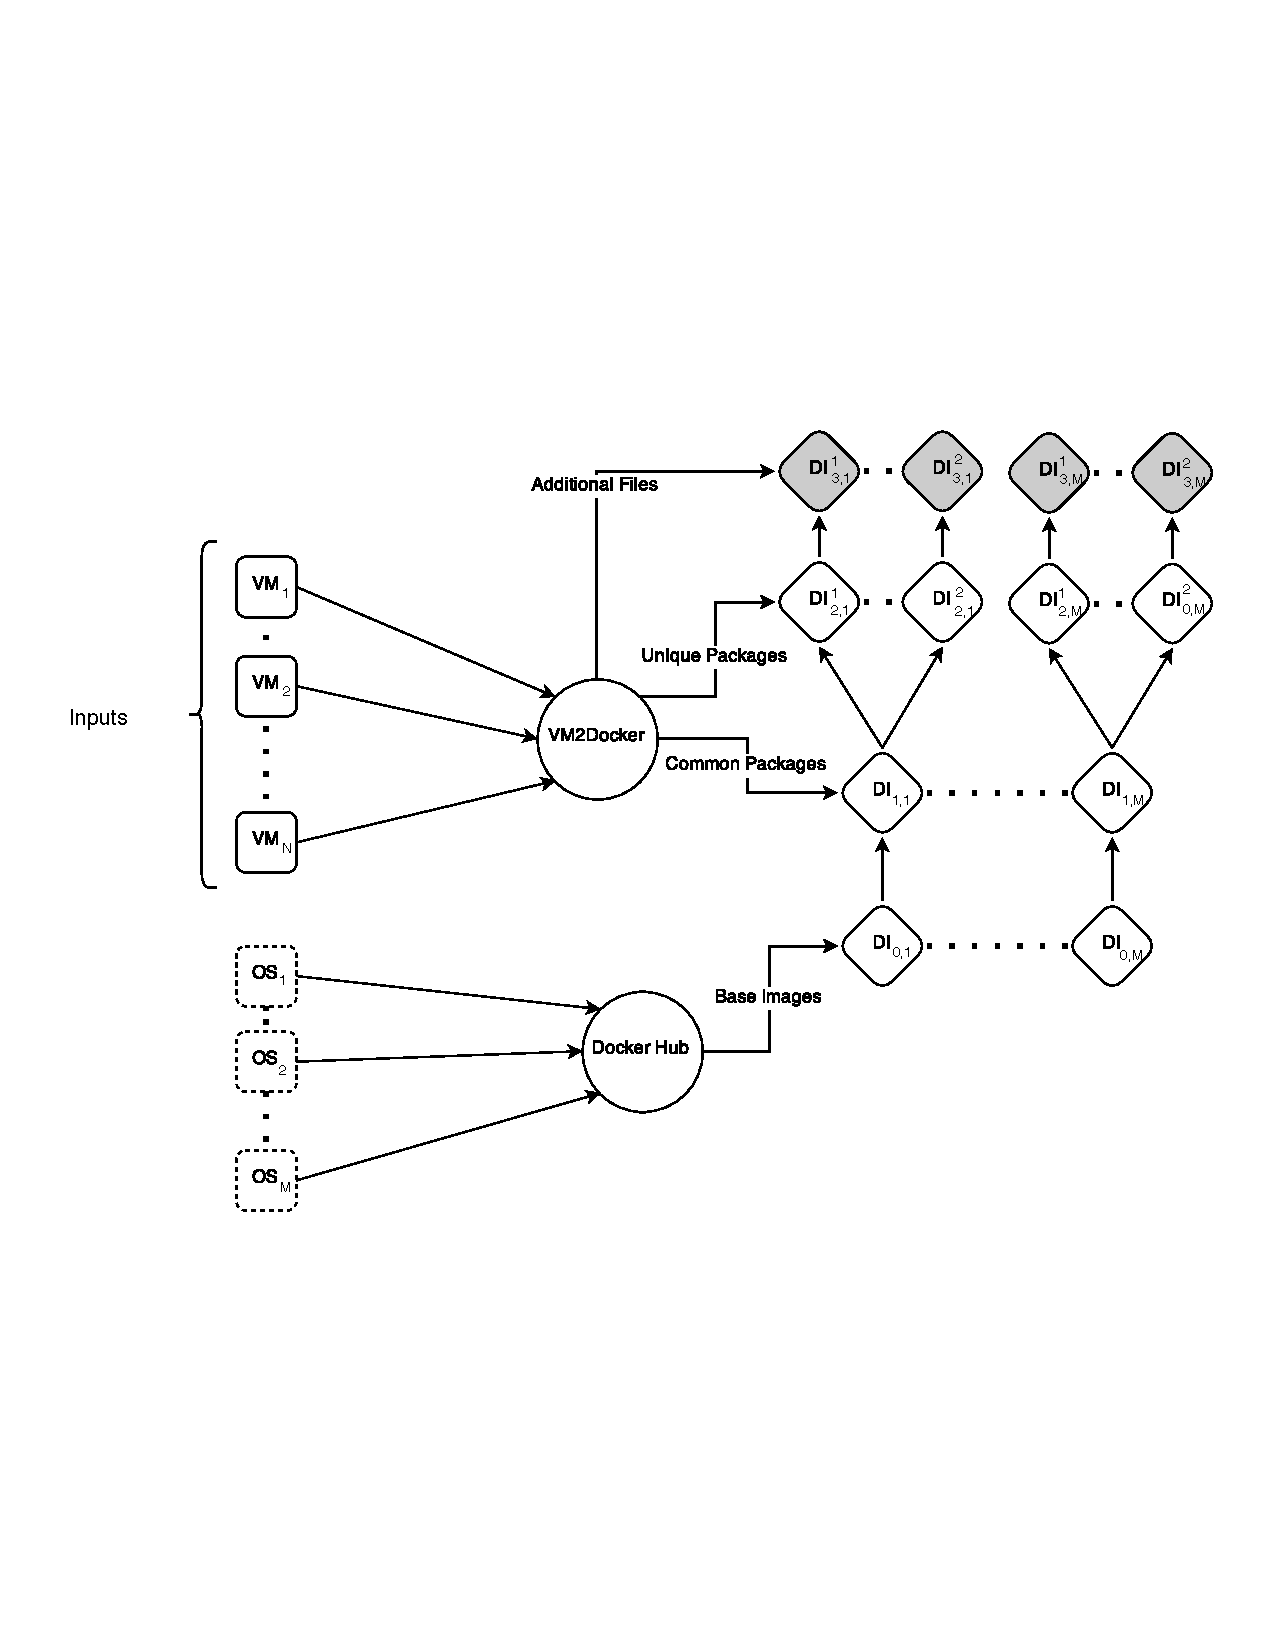
\includegraphics[width=1.0\textwidth]{system.pdf}
    \caption{The following diagram illustrates an overview of the system and how the VM2Docker framework interacts with the virtual machines provided as input and converts them to corresponding, layered, Docker containers. The rounded squares represent the input virtual machines, the circles correspond to immutable programs that interact with the inputs or outputs in some way, and the rounded diamonds represent the resulting Docker images. Each image consists of a series of layers, which is illustrated by starting at the given image and traversing the links backwards to the base image ($DI_0$). The final images, equal to the original VM filesystem, are represented by the shaded diamonds ($DI_3$). The number of these is exactly equal to N, the original number of VMs to be converted.}
\label{fig:systemeval}
\end{figure}
%$\text{DC}_3$)
% ($\text{DC}_0$)

\subsubsection{Single VM Conversions}
For the following set of experiments, we will assume that $N=1$ in the following diagram. By extension, this also implies that $M=1$. In practice, this reduces the effectiveness and utility of the system as a whole. As we will see, there is a tradeoff between increased layering and increased aggregate image size. VM2Docker generally favors the former at the expense of the latter, but the benefits of the former are not fully realized without multiple virtual machines present. As a result, converting a single virtual machine, while supported, is less optimal and is done purely as a theoretical analysis of the relative size of layers that VM2Docker can produce for a wide range of inputs.

We start by analyzing the results of running a single, vanilla install of a Linux operating system through VM2Docker with package management disabled. These virtual machine installers were obtained through the respective software websites are available for public download. With package management disabled, the view of layers produced for a given virtual machine is collapsed to $DI_0$ and $DI_3$. There is also a Dockerfile, which we will denote $DF$, that provides the instructions and additional data to the Docker engine of how to build $DI_3$ from $DI_0$. While the total size of $DI_3$ is by definition the same regardless of which diff algorithm is used, as we will see, the size of the delta file and therefore $DF$ can vary. Thus, the size of $DF$ and $DI_3$ are therefore important metrics in determining the speed of deployment and disk space required while running, respectively. We assume for the sake of consistency, that all sizes are provided, uncompressed. In practicality, the Docker engine likely automatically makes use of compression on both sides of a given download of an image. We therefore leave that topic as one beyond the scope of this paper and simply acknowledge this omission.

We use the term, bare VM, to denote a virtual machine, not including kernel files and other cache files that may be removed, as mentioned in section~\ref{sec:addnltechs}. This exclusion allows us to focus on benefits and drawbacks of our layering strategy without confounding the results of the strict benefits of excluding the kernel files, which would not be used inside of the Docker framework.

Tables~\ref{table:diff},~\ref{table:diff2}, and~\ref{table:diff3} show the results of these conversions. As we see, \texttt{rdiffdir} generally provides a slightly more compact delta file as compared to the \texttt{rsync} alternative. However, due to the dependencies of the \texttt{rdiffdir} package itself, as discussed in section~\ref{sec:rdiffdir}, the rsync algorithm is generally simpler and more straightforward to analyze. Furthermore, the byte representation of the the \texttt{rsync} diff file (a tarball of changes and modifications) maps directly to the size of $DI_3$, so it is simpler to use these interchangeably in our discussion.

In many cases, the aggregate size of all layers is no smaller than the original bare VM size. Overall, as introduce more and more layers from package management, the size of $DI_3$ decreases. This implies that some increase in the size of $DI_0+DI_1 + DI_2$, $x$, results in a decrease in the size of $DI_3$, $y$, where $|x| \ge |y|$. These results are an example of the size to layering tradeoff mentioned at the beginning of this subsection. To better quantify this tradeoff, we introduce two important quantities that will be used throughout the evaluation process. 

First, we introduce a measure of the total space used in all layers up to and including layer $i$. This metric, $\Phi_i$, is defined as:

\begin{equation}
\Phi_i = \sum_{j=0}^i DI_j
\end{equation}

Throughout our discussion of single VM conversions without package management, $\Phi_1$ is the only additional value of interest, since $DI_2=DI_3=0$ so $\Phi_1=\Phi_2=\Phi_3$. When we incorporate package management, $DI_2 \neq 0$ and then with multiple VM conversions $DI_3 \neq 0$. These values will help quantify the fixed cost of increased layering at different locations in the inheritance tree for the first such VM to be converted. 

We also define a metric, $\Xi$, as the minimum whole number of VMs needed in order to achieve the goal of aggregate space savings. As we will see, $\Xi$ increases as we add more aggressive package management detection, but this also decreases $DI_3$, which can be thought of as the marginal cost of an additional VM of the particular OS and release. Theoretically, $\Xi$ can be defined at multiple layers of the inheritance tree, depending on which packages certain VMs share in common. For example, two VMs may share the same OS and release, and some but not all of the same packages installed. In this case, they would share $DI_0$ and $DI_1$ in common. In other cases, certain VMs might only differ in their filesystem composition, and could therefore share up to $DI_2$ in common. Thus, we consider $\Xi_i$ as the minimum whole number of VMs needed to achieve the goal of aggregate space savings, where the VMs share up to layer $i$ in common. This value can be attained by solving the following inequality for the smallest possible whole number value, $\Xi_i$.

In the equations below, we define $\beta$ as the size of the Bare VM.

\begin{equation}
\Phi_i + (\Phi_3 - \Phi_i)* \Xi_i \le \Xi_i * \beta
\end{equation}

However, for simplicity, we consider only this value when all packages are shared in common, and the $DI_3$ layer is different. Therefore, formally, $\Xi = \Xi_2$ can be simplified to the following:

\begin{align*}
\Phi_i + (\Phi_3 - \Phi_i)* \Xi_i &\le \Xi_i * \beta \\
\Phi_2 + (\Phi_3 - \Phi_2)* \Xi_2 &\le \Xi_2 * \beta \\
\Phi_2 + (DI_3)* \Xi &\le \Xi * \beta\\
\Xi &\ge \frac{\Phi_2}{\beta - DI_3} \\
\Xi &= \ceil*{\frac{\Phi_2}{\beta - DI_3}}
\end{align*}

%TODO!!: consider reorganizing equations to go before the start of the single VM conversions section

In the results, the layering tradeoff is very minimal while making use of only filesystem diffs. With $\Xi =2$ for all OS releases tested, we see that the presence of even a single additional container image of the same OS and release ensures that the layering strategy introduced by Docker not only breaks up the VM into more logical, deployable components but also saves space in the process.

\begin{table}[h]
\centering
    \begin{tabular}{| c | c | c | c | c | c | c |}
    \hline
& \multicolumn{5}{|c|}{\bfseries Ubuntu Server} \\ \hline
    \bfseries Release & \itshape 12.04 & \itshape 13.04 & \itshape 13.10 & \itshape 14.04 & \itshape 14.10 \\ \hline
    \bfseries Bare VM ($\beta$) & 1023.5 & 774.1 & 1055.2 & 1109.9 & 1029.9\\ \hline
    \bfseries Base Image ($DI_0$) & 99.1 & 160.4 & 174.6 & 192.0 & 196.9  \\ \hline
    \bfseries rsync & 956.7 & 730.9 & 963.6 & 1008.9 & 876.4\\ \hline 
    \bfseries rdiff & 934.4 & 738.2 & 957.3 & 971.2 & 872.5\\ \hline 
    \bfseries $\boldsymbol{\Xi}$ & 2 & 2 & 2 & 2 & 2  \\ \hline
    \end{tabular}
\caption{The results of running VM2Docker with a single VM input and various releases of Ubuntu. The \texttt{rdiff} algorithm generall provides slightly smaller delta files. For all inputs, $\Xi = 2$ and therefore space savings begin to occur on the second instance of a given OS release.}
\label{table:diff}
\end{table}

\begin{table}[h]
\centering
    \begin{tabular}{| c | c | c | c |}
    \hline
& \multicolumn{3}{|c|}{\bfseries CentOS Minimal} \\ \hline
    \bfseries Release & \itshape 5* & \itshape 6 & \itshape 7 \\ \hline
    \bfseries Bare VM ($\beta$) & 2441.5 &  618.2 & 779.4\\ \hline
    \bfseries Base Image ($DI_0$) & 496.0 & 236.1 & 243.1\\ \hline
    \bfseries rsync & 2190.0 & 450.1 & 601.8\\ \hline 
    \bfseries rdiff & 2138.7 & 416.7 & 519.4\\ \hline
\bfseries $\boldsymbol{\Xi}$ & 2 & 2 & 2 \\ \hline
    \end{tabular}
\caption{The results of running VM2Docker with a single VM input and various releases of CentOS. The \texttt{rdiff} algorithm generall provides slightly smaller delta files. For all inputs, $\Xi = 2$ and therefore space savings begin to occur on the second instance of a given OS release.}
\label{table:diff2}
\end{table}

\begin{table}[h]
\centering
    \begin{tabular}{| c | c | c |}
    \hline
& \multicolumn{2}{|c|}{\bfseries Mageia} \\ \hline
    \bfseries Release & \itshape 3 & \itshape 4*  \\ \hline
    \bfseries Bare VM ($\beta$) & 636.1 & 2706.1 \\ \hline
    \bfseries Base Image ($DI_0$) & 160.4 & 174.1\\ \hline
    \bfseries rsync & 525.1 & 2575.4\\ \hline 
    \bfseries rdiff & 511.0 & 2613.0\\ \hline 
\bfseries $\boldsymbol{\Xi}$ & 2 & 2  \\ \hline
    \end{tabular}
\caption{The results of running VM2Docker with a single VM input and various releases of Mageia. The \texttt{rdiff} algorithm generall provides slightly smaller delta files. For all inputs, $\Xi = 2$ and therefore space savings begin to occur on the second instance of a given OS release. The * denotes that VM2Docker was run on the fullly featured release of this OS with all default packages installed, which explains the increase in overall size of the input VM.}
\label{table:diff3}
\end{table}

We next continue the analysis of these basic, vanilla linux VMs by enabling the use of package management. We therefore now also consider the size of an additional layer, $DI_1$, in our discussion. For simplicity, we assume we are only using \texttt{rsync} as our preferred method of filesystem diff, and label this $DI_3$.

As shown in tables~\ref{table:diffpm} and~\ref{table:diffpm2}, when package management is enabled in VM2Docker we observe a few important trends. First, the size of $DI_3$ decreases as a result of the existence of $DI_1$. This makes sense and is expected because the package management logic allows for some of the filesystem space occupied by packages that was formerly stored in the filesystem diff to be extracted downwards into $DI_1$. A consequence of this is that the total size of all layers, $\Phi_3$, also increases. However, overall this tradeoff is considered acceptable and preferred because $\Xi$ remains fixed at 2 and the overall layering and therefore deployability of each container increases.

When analyzing the overall results of these base case experiments and the layering results of converting a single virtual machine at a time, we take a step back and consider the efficiency of these outcomes. An optimal conversion would be one such that the size of $DI_3$ is as close to 0 as possible. This would imply that the package extraction and reinstallation process is 100\% effective and is able to fully account for all or almost all files within a VM. The implications of such a container would be that the vanilla VMs would be fully "Dockerized." In practice, however, the size of $DI_3$ is far from zero, although the resulting sizes are still greatly reduced from the size of the original bare VM. There are a few practical limitations of the package detection and reinstallation process that can account for these results. Due to the automatic detection of packages and reinstallation on top of $DI_0$ with auto-generated commands, it is likely that some, but not all, of the packages that are reinstalled are not identical byte-for-byte versions of the original packages that were installed on the VM. This can be due to a difference in version number, release, or some other subtle difference in the installation process. This would result in some or all of a given package to still exist in the ``additional files" component of $DI_3$. There is also a host of software and files that can't necessarily be reinstalled from the default package management tool for the given OS. Cache files, too, can sometimes account for 50-100 MB of files in the original VM.

This point of comparison is used to quantify the percentage reduction in the marginal cost of deploying an additional VM, before and after the VM2Docker framework has performed the automatic layering. In tables~\ref{table:diffpm} and~\ref{table:diffpm2}, this value is represented by the symbol $\chi$ and is shown to range from 15.8 to 56.5.
 
% data tables that include package installation
\begin{table}[h]
\centering
    \begin{tabular}{| c | c | c | c | c |}
    \hline
& \multicolumn{4}{|c|}{\bfseries Ubuntu Server} \\ \hline
    \bfseries Release & \itshape 12.04 & \itshape 13.10 & \itshape 14.04 & \itshape 14.10 \\ \hline
    \bfseries Bare VM ($\beta$) & 1023.5  & 1055.2 & 1109.9 & 1029.9\\ \hline
    \bfseries $\boldsymbol{DI_0}$ & 99.1 & 174.6 & 192.0 & 196.9  \\ \hline
    \bfseries $\boldsymbol{DI_1}$ & 227.3 & 273.7 & 194.9 & 271.7  \\ \hline
    \bfseries $\boldsymbol{DI_3}$ & 862.2 & 733.7 & 894.8 & 687.6\\ \hline 
\bfseries $\boldsymbol{\chi}$ & 15.8 & 30.5 & 19.4 & 33.2\\ \hline 
     \bfseries $\boldsymbol{\Phi_3}$ & 1188.6 & 1182.0 & 1281.7 & 1156.2\\ \hline
\bfseries $\boldsymbol{\Xi}$ & 2 & 2 & 2 & 2\\ \hline
    \end{tabular}
\caption{The results of running VM2Docker with a single VM input and various releases of Ubuntu. As the overall layering increases, the size of $DI_3$ decreases, which results in a increasing \% overall reduction, $\chi$ in the marginal cost of deploying a given VM. For all inputs, $\Xi = 2$ and therefore space savings begin to occur on the second instance of a given OS release.}
\label{table:diffpm}
\end{table}

\begin{table}[h]
\centering
    \begin{tabular}{| c | c | c | c |}
    \hline
& \multicolumn{2}{|c|}{\bfseries CentOS} & \multicolumn{1}{|c|}{\bfseries Mageia} \\ \hline
    \bfseries Release & \itshape 6 & \itshape 7 & \itshape 3 \\ \hline
    \bfseries Bare VM ($\beta$) & 618.2 & 779.4 & 636.1\\ \hline
    \bfseries $\boldsymbol{DI_0}$ & 236.1 & 243.1 & 160.4  \\ \hline
    \bfseries $\boldsymbol{DI_1}$ & 244.0 & 417.1 & 544.2 \\ \hline
    \bfseries $\boldsymbol{DI_3}$ & 380.5 & 339.9 & 465.9 \\ \hline
\bfseries $\boldsymbol{\chi}$ & 38.5 & 56.5 & 26.8 \\ \hline
     \bfseries $\boldsymbol{\Phi_3}$ & 860.6 & 1000.1 & 1170.5 \\ \hline
     \bfseries $\boldsymbol{\Xi}$ & 2 & 2 & 2 \\ \hline
    \end{tabular}
\caption{The results of running VM2Docker with a single VM input and various releases of CentOS and Mageia. As the overall layering increases, the size of $DI_3$ decreases, which results in a increasing \% overall reduction, $\chi$ in the marginal cost of deploying a given VM. For all inputs, $\Xi = 2$ and therefore space savings begin to occur on the second instance of a given OS release.}
\label{table:diffpm2}
\end{table}


%TODO: discussion here about these threshold numbers for number of VMs for package management to make sense. etc. 


\subsubsection{Multiple VM Conversions}
\label{sec:multivm}
For the following set of experiments, we will assume that $M=1$ in figure~\ref{fig:systemeval}. This will greatly reduce the number of experiments to be run as well as simplify the understanding of the system diagram in each case. Each distinct operating system does not share any resulting image layers in common because the first layer, the base image ($DI_0$), is OS and release-specific. Thus, restricting our set of inputs such that all VMs share the same OS and release ($M=1$) does not drastically alter the results and instead represents a narrowing of scope to a single tree of image layers, pictured on the right in figure~\ref{fig:systemeval}. The results for $M>1$ can be therefore obtained by merging the results from a set of $M$ independent experiments each of which $M=1$.

We therefore seek to analyze various combinations of VM inputs of a given OS and release, each with different package and file compositions. These results will provide material support for the theoretical calculations done in the previous section. In all experiments so far, it was determined that only a second additional VM was needed in order to establish total space savings as compared to not using the VM2Docker system at all. Thus, these multiple VM experiments, for simplicity, will only have 2 or 3 total VMs provided as input, but we argue that the scenarios chosen are highly representative of the types of combinations and subsets of VMs VM2Docker might need to handle. Furthermore, as the number of VMs of a given OS and release increases, the overall space savings will increase, as argued in the previous section.

It is challenging to describe what might be an "average" looking input to this system because one could use a virtual machine to do a wide range of computing. Nonetheless, there are many real-world practical use cases where VM2Docker might be particularly effective. The class of VMs that are used as servers in a simple client-server interaction are one example of such inputs. A given VM might be running a webserver, database, mail server, or other server-based daemon and might represent one such input to the VM2Docker system. 

We have designed a total of five experiments with various characteristics and combinations of input VMs in order to highlight strengths and weaknesses of the overall algorithm and framework. For each scenario, we begin by describing how we expect VM2Docker to handle these inputs in terms of the expected size of the outputs. These experiment descriptions will be OS-agnostic. We next present the results of running this experiment for specific releases of multiple OS's (Ubuntu, CentOS, and Mageia). 
%Finally, we discuss any findings that might be unexpected or out of the ordinary.

\begin{enumerate}
\item \underline{Scenario A}\\
\textit{Input}:\\
$\boldsymbol{VM_1}$: Minimal OS, $\sim$ 1GB \textemdash\ $\boldsymbol{VM_2}$: OS Complete Install, $\sim$ 2-3GB\\

The difference between these two VMs is additional packages and repositories that are provided in the complete install. The second VM will contains all of the packages on the first VM, as well as a few gigabytes of additional software.


\textit{Expected Output}:
%$DC_1$: 286.5 MB\\
%$DC_2^1$: 0 MB\\
%$DC_2^2$: $\sim$ 1.5 - 2 GB\\
%$DC_3^1$: 157.1MB\\
%$DC_3^2$: 300-500MB\\

With two VMs provided as input, they will each share the same base image $DI_0$ for the given OS release. The next layer, $DI_1$, will also be common to the two containers and will contain all the packages common to the two VMs. At this point, the inheritance tree will split into two, one branch for each of the two provided inputs. $DI_1$ will be exactly the same size as the original $DI_1$ from the single VM experiments. $DI_2^1$ will be an empty layer that occupies no space, because there are no packages in $VM_1$ that are not also in $VM_2$. $DI_2^2$ will take up a few GB as it will be where all of the packages unique to $VM_2$ are located. Finally, $DI_3^1$ will be the same size as its corresponding layer in the original experiments and $DI_3^1$ we can expect to be larger as it will contain the remainder of the packages and their associated files not also installed in the previous layer.

\begin{table}[h]
\centering
    \begin{tabular}{| c | c | c | c|}
    \hline
    \bfseries Release & \itshape Ubuntu 13.10 & \itshape CentOS 6 & \itshape Mageia 3\\ \hline
\bfseries $\boldsymbol{VM_1}$ & 1055.2 & 618.2 & 636.1\\ \hline
\bfseries $\boldsymbol{VM_2}$ & 3232.4 & 2051.1 & 1669.4\\ \hline \hline
    \bfseries $\boldsymbol{DI_1}$ & 273.7 & 244.0 & 544.2\\ \hline
    \bfseries $\boldsymbol{DI_2^1}$ & 0 & 0 & 0\\ \hline 
\bfseries $\boldsymbol{DI_2^2}$ & 2092.1 & 490.8 & 898.1\\ \hline 
\bfseries $\boldsymbol{DI_3^1}$  & 733.7 & 380.5 & 465.9\\ \hline 
\bfseries $\boldsymbol{DI_3^2}$ & 1646.1 & 1541.9 & 1225.3\\ \hline 
    \end{tabular}
\caption{The results of running the multi VM scenario A with M=1. All values are in MB.}
\label{table:multiscenarioa}
\end{table}



\item \underline{Scenario B}\\
\textit{Input}:\\
$\boldsymbol{VM_1}$: Minimal OS, $\sim$ 1GB \textemdash\ $\boldsymbol{VM_2}$: Minimal OS + 300MB additional files, $\sim$ 1GB\\

\textit{Expected Output}:

%$DC_1$: 286.5 MB\\
%$DC_2^1$: 0 MB\\
%$DC_2^2$: 0 MB\\
%$DC_3^1$: 157.1MB\\
%$DC_3^2$: 457MB\\

The only differences between these two VMs comes in the addition of 300MB of files that can't be categorized into packages. This will result in an increase in $DI_3^2$ of the size of the additional files that were added to the VM. All other values should be the same as those in the single VM experiments.

\begin{table}[h]
\centering

    \begin{tabular}{| c | c | c | c|}
    \hline
    \bfseries Release & \itshape Ubuntu 13.10 & \itshape CentOS 6 & \itshape Mageia 3\\ \hline
\bfseries $\boldsymbol{VM_1}$ & 1055.2 & 618.2 & 636.1\\ \hline
\bfseries $\boldsymbol{VM_2}$ & 1355.2 & 918.2 & 936.1\\ \hline \hline
    \bfseries $\boldsymbol{DI_1}$ & 273.7 & 244.0 & 544.2\\ \hline
    \bfseries $\boldsymbol{DI_2^1}$ & 0 & 0 & 0\\ \hline 
\bfseries $\boldsymbol{DI_2^2}$ & 0 & 0 & 0\\ \hline 
\bfseries $\boldsymbol{DI_3^1}$  & 733.7 & 380.5 & 465.9\\ \hline 
\bfseries $\boldsymbol{DI_3^2}$ & 1033.7 & 680.5 & 765.9\\ \hline 
    \end{tabular}
\caption{The results of running the multi VM scenario B with M=1. All values are in MB.}
\label{table:multiscenariob}
\end{table}


\item \underline{Scenario C}\\
\textit{Input}:\\
$\boldsymbol{VM_1}$: Minimal OS, $\sim$ 1GB \textemdash\ $\boldsymbol{VM_2}$: Minimal OS + 300MB additional files, $\sim$ 1GB \textemdash $\boldsymbol{VM_3}$: OS Complete Install, $\sim$ 2-3GB\\

\textit{Expected Output}:

%$DC_1$: 286.5 MB\\
%$DC_2^1$: 0 MB\\
%$DC_2^2$: 0 MB\\
%$DC_2^3$: $\sim$ 1.5 - 2 GB\\
%$DC_3^1$: 157.1MB\\
%$DC_3^2$: 457MB\\
%$DC_3^3$: 300-500MB\\

These results should be a combination of the two previous two experiments, with the sizes remaining the same as if the experiments were run separately. 
\begin{table}[h]
\centering

    \begin{tabular}{| c | c | c | c|}
    \hline
    \bfseries Release & \itshape Ubuntu 13.10 & \itshape CentOS 6 & \itshape Mageia 3\\ \hline
\bfseries $\boldsymbol{VM_1}$ & 1055.2 & 618.2 & 636.1\\ \hline
\bfseries $\boldsymbol{VM_2}$ & 1355.2 & 918.2 & 936.1\\ \hline
\bfseries $\boldsymbol{VM_3}$ & 3232.4 & 2051.1 & 1669.4\\ \hline \hline
    \bfseries $\boldsymbol{DI_1}$ & 273.7 & 244.0 & 544.2\\ \hline
    \bfseries $\boldsymbol{DI_2^1}$ & 0 & 0 & 0\\ \hline 
\bfseries $\boldsymbol{DI_2^2}$ & 0 & 0 & 0\\ \hline 
\bfseries $\boldsymbol{DI_2^3}$ & 2092.1 & 490.8 & 898.1\\ \hline 
\bfseries $\boldsymbol{DI_3^1}$  & 733.7 & 380.5 & 465.9\\ \hline 
\bfseries $\boldsymbol{DI_3^2}$ & 1033.7 & 680.5 & 765.9\\ \hline 
\bfseries $\boldsymbol{DI_3^3}$ & 1646.1 & 1541.9 & 1225.3\\ \hline 
    \end{tabular}
\caption{The results of running the multi VM scenario C with M=1. All values are in MB.}
\label{table:multiscenarioc}
\end{table}


\item \underline{Scenario D}\\
\textit{Input}:\\
$\boldsymbol{VM_1}$: Minimal OS, $\sim$ 1GB \textemdash\ $\boldsymbol{VM_2}$: OS Complete Install + 300MB additional files, $\sim$ 2-3GB \textemdash $\boldsymbol{VM_3}$: OS Complete Install, $\sim$ 2-3GB\\

%$VM_1$: CentOS6 Minimal, 676 MB\\
%$VM_2$: CentOS6 Complete plus 300 MB of additional files scattered across the OS, 3.1GB\\
%$VM_3$: CentOS6 Complete, 2.8 GB\\

\textit{Expected Output}:

%$DC_1$: 286.5 MB\\
%$DC_2^1$: 0 MB\\
%$DC_2^2$: $\sim$ 1.5 - 2 GB\\
%$DC_2^3$: $\sim$ 1.5 - 2 GB\\
%$DC_3^1$: 157.1MB\\
%$DC_3^2$: 600-800MB\\
%$DC_3^3$: 300-500MB\\

These results should be similar in practice to the previous experiment as well. An interesting feature of VM2Docker will be exposed here as well. Since $DI_2^2$ and $DI_2^3$ are the same, they will be only represented once on disk by the same image. This is thanks to an implicit feature of Docker. Since VM2Docker generates Dockerfiles, which are instructions to generate the image, the Dockerfiles for $DI_2^2$ and $DI_2^3$ will be the same (the commands are the same and they are installing the same packages). VM2Docker sorts the list of packages being installed alphabetically to ensure that the command in the Dockerfile is the same on subsequent runs. 

\begin{table}[h]
\centering

    \begin{tabular}{| c | c | c | c|}
    \hline
    \bfseries Release & \itshape Ubuntu 13.10 & \itshape CentOS 6 & \itshape Mageia 3\\ \hline
\bfseries $\boldsymbol{VM_1}$ & 1055.2 & 618.2 & 636.1\\ \hline
\bfseries $\boldsymbol{VM_2}$ & 3532.4 & 2351.1 & 1969.4\\ \hline
\bfseries $\boldsymbol{VM_3}$ &  3232.4 & 2051.1 & 1669.4\\ \hline \hline
    \bfseries $\boldsymbol{DI_1}$ & 273.7 & 244.0 & 544.1\\ \hline
    \bfseries $\boldsymbol{DI_2^1}$ & 0 & 0 & 0\\ \hline 
\bfseries $\boldsymbol{DI_2^2}$ & 2092.1 & 490.8 & 898.1\\ \hline 
\bfseries $\boldsymbol{DI_2^3}$ & 2092.1 & 490.8 & 898.1\\ \hline 
\bfseries $\boldsymbol{DI_3^1}$  & 733.7 & 380.5 & 465.9\\ \hline 
\bfseries $\boldsymbol{DI_3^2}$ & 1946.1 & 1841.9 & 1525.3\\ \hline 
\bfseries $\boldsymbol{DI_3^3}$ & 1646.1 & 1541.9 & 1225.3\\ \hline 
    \end{tabular}
\caption{The results of running the multi VM scenario D with M=1. All values are in MB.}
\label{table:multiscenariod}
\end{table}

\item \underline{Scenario E}\\
\textit{Input}:\\
$\boldsymbol{VM_1}$: Minimal OS, $\sim$ 1GB \textemdash\ $\boldsymbol{VM_2}$: OS Complete Install, $\sim$ 2-3GB \textemdash $\boldsymbol{VM_3}$: OS Complete Install + Ruby, $\sim$ 2-3GB\\

%$VM_1$: CentOS6 Minimal, 676 MB\\
%$VM_2$: CentOS6 Complete, 2.8 GB\\
%$VM_3$: CentOS6 Complete plus 1 more package of negligible size, 2.8 GB\\

\textit{Expected Output}:

%$DI_1$: 286.5 MB\\
%$DI_2^1$: 0 MB\\
%$DI_2^2$: $\sim$ 1.5 - 2 GB\\
%$DI_2^3$: $\sim$ 1.5 - 2 GB\\
%$DI_3^1$: 157.1MB\\
%$DI_3^2$: 600-800MB\\
%$DI_3^3$: 300-500MB\\

These results will be the same as in the previous experiment, except that $DI_2^2$ and $DI_2^3$ will no longer occupy the same space on disk and will be two distinct images. The Ruby package itself is no more than 10-20MB, the end result will be more than 2GB additional space used on disk. This reveals a shortcoming of VM2Docker in its inability to execute multiple rounds of finding packages in common between multiple VMs. This will be addressed further in the discussion and future work section.
\begin{table}[h]
\centering

    \begin{tabular}{| c | c | c | c|}
    \hline
    \bfseries Release & \itshape Ubuntu 13.10 & \itshape CentOS 6 & \itshape Mageia 3\\ \hline
\bfseries $\boldsymbol{VM_1}$ & 1055.2 & 618.2 & 636.1\\ \hline
\bfseries $\boldsymbol{VM_2}$ & 3232.4 & 2051.1 & 1669.4\\ \hline
\bfseries $\boldsymbol{VM_3}$ &  3245.4 & 2063.8 & 1680.2\\ \hline \hline
    \bfseries $\boldsymbol{DI_1}$ & 273.7 & 244.0 & 544.2\\ \hline
    \bfseries $\boldsymbol{DI_2^1}$ & 0 & 0 & ??\\ \hline 
\bfseries $\boldsymbol{DI_2^2}$ & 2092.1 & 490.8 & 898.1\\ \hline 
\bfseries $\boldsymbol{DI_2^3}$ & 2104.9 & 502.1 & 909.3\\ \hline 
\bfseries $\boldsymbol{DI_3^1}$  & 733.7 & 380.5 & 465.9\\ \hline 
\bfseries $\boldsymbol{DI_3^2}$ & 1646.1 & 1541.9 & 1225.3\\ \hline 
\bfseries $\boldsymbol{DI_3^3}$ & 1647.3 & 1542.3 & 1225.8\\ \hline 
    \end{tabular}
\caption{The results of running the multi VM scenario E with M=1. All values are in MB.}
\label{table:multiscenarioe}
\end{table}

\end{enumerate}


Overall, VM2Docker performs as expected when combining the single VM experiments with various combinations of VMs from the same OS and release. Of interest is the ability with which each of the given operating system's reinstallation process effectively reduces the size of $DI_3$. Relative to the size of the original VM, it seems as if CentOS 6 had the smallest $DI_2$ layer, while still being able to reduce the size of $DI_3$. Furthermore, Ubuntu 13.10 seems to have the largest reduction from original bare VM size to $DI_3$, but $DI_2$ is also the largest for this OS, so it comes at a fixed cost. Of course, this fixed cost is made up for after the second VM is converted, as is the case in scenario D. Thus, as a whole we argue that these experimental results support the argument that the introduction of automatic layering by base image, packages, and filesystem diff and serves to reduce the overall space used by the containers as compared to the original VMs, as long as $\Xi \ge 2$. 



\subsection{Dependency Detection}
We now present the experimental results of applying the dependency detection algorithm mentioned in section~\ref{sec:depdetection}. The results are even better than expected, as shown in table~\ref{table:culling}, suggesting that a relatively high percentage of the packages installed for a given OS and release are actually dependencies of others. During the installation process, most package management tools will automatically resolve the dependencies of a desired piece of software, therefore enabling the removal of these dependencies from the list of software to be installed in a given Dockerfile. Overall, simplicity and readability of a Dockerfile is always beneficial, as it allows for more transparent exposure of the steps involved in the build process of a given Docker image.

\begin{table}[h]
\centering

    \begin{tabular}{| c | c | c | c | c | c | c | c | c |}
    \hline
& \multicolumn{5}{|c|}{\bfseries Ubuntu Server} & \multicolumn{2}{|c|}{\bfseries CentOS} & \multicolumn{1}{|c|}{\bfseries Mageia} \\ \hline
    \bfseries Release & \itshape 12.04 & \itshape 13.04 & \itshape 13.10 & \itshape 14.04 & \itshape 14.10  & \itshape 6 & \itshape 7 & \itshape 3 \\ \hline
    \bfseries Before & 205 & 226 & 248 & 183 & 245 & 78 & 165 & 311\\ \hline
    \bfseries After & 67 & 129 & 147 & 109 & 144 & 54 & 67 & 46   \\ \hline \hline
    \bfseries \% Saved & 67.3 & 42.9 & 40.7 & 40.4 & 41.2 & 30.8 & 59.4 & 85.2\\
    \hline
    \end{tabular}
\caption{The results show a fairly aggressive reduction of packages required to be listed across many different operating systems and releases. Of the original packages to be installed, as many as 85.2\% and as few as 30.8\% can be removed without affecting the overall set of packages.}
\label{table:culling}
\end{table}

\section{Qualitative Results}
\label{sec:evalqual}
\subsection{OS Compatibility}
VM2Docker is written with the intent of supporting all potential operating systems a given VM might be running. OS-specific implementation details are largely limited to the package management features provided by VM2Docker to increase the number of generated layers. Each OS uses a particular package management tool, with its own command signature and behavior. VM2Docker must be capable of generating instructions to install and uninstall packages for the given OS. Furthermore, to support the culling of packages and the automatic dependency detection, each OS must be capable of dynamically determining the dependencies for a given package.

As a result, the following four commands must be provided for each additional package management tool that requires support. 
\begin{enumerate}
\item Get list of installed packages
\item Install the given packages
\item Uninstall the given packages
\item Get the dependencies for a given package
\end{enumerate}

We now discuss how these commands were implemented for the various operating systems tested.

\subsubsection{Ubuntu}
Ubuntu uses \texttt{dpkg} and \texttt{apt-get} as its package management tool. The following commands were therefore defined in order to provide support for Ubuntu:
\begin{enumerate}
\item \texttt{dpkg --get-selections}
\item \texttt{apt-get install \%s}
\item \texttt{apt-get remove \%s}
\item \texttt{apt-cache depends \%s | grep ``Depends:''}
\end{enumerate}
\subsubsection{CentOS}
CentOS uses the \texttt{yum} package manager as its package management tool. The following commands were therefore defined in order to provide support for CentOS.
\begin{enumerate}
\item \texttt{rpm -qa --queryformat `\%\{NAME\}\textbackslash n'}
\item \texttt{yum -y install \%s}
\item \texttt{yum -y erase \%s}
\item \texttt{repoquery --requires --resolve \%s --qf \%\{NAME\}}
\end{enumerate}

Additionally, as of CentOS 7, there is a built-in firewall in the OS that interferes with the VM2Docker agent and its ability to accept socket connections from external clients (the chief). For this particular build of Linux, the firewall is managed by the \texttt{firewall-cmd} command, and therefore an exception was required to be granted over TCP for the appropriate port (by default 49153).

\subsubsection{Mageia}
Mageia uses the \texttt{urpmi} package manager as its package management tool. The following commands were therefore defined in order to provide support for Mageia in VM2Docker.

\begin{enumerate}
\item \texttt{rpm -qa --queryformat `\%\{NAME\}\textbackslash n'}
\item \texttt{urpmi --auto \%s}
\item \texttt{urpme \%s}
\item \texttt{urpmq -d \%s}
\end{enumerate}

Additionally, similar to CentOS 7, Mageia provides a firewall, called Shorewall, that is enabled by default and prevents the VM2Docker agent to accept socket connections from external clients (the chief). For this particular build of Linux, the firewall is managed by the \texttt{iptables} command, and therefore an exception was required to be granted over TCP for the appropriate port (by default 49153).

As a whole, VM2Docker attempts to provide seamless and simplified support for any Linux-based operating system. While many components of the conversion process are OS-agnostic, such as the Docker-based host initiating the conversion, the overall filesystem benefits of detecting package dependencies outweigh the costs of supporting a wide range of package management tools. The 3-4 commands that must be provided for full package management support are, in our opinion, a minimal one-time configuration cost in order to harness the full-layering benefits of the VM2Docker conversion process.

\subsection{Conversion Time}
There are a number of different factors that can drastically impact the overall conversion time of the virtual machines provided as input. In particular, as the number of input VMs increases, the overall time increases proportionally as each VM is processed, one at a time, after the package intersection step. Another important determinant of conversion time is the time the hard drive is in use when calculating and applying the filesystem diff. Solid state drives provide an incredible performance improvement over a spinning disk hard drive during the filesystem diff generation process. In practice, the diff operation was slowed down by almost an entire order of magnitude on a hard disk as compared to an SSD. In addition to hard drive speed, network speed also becomes a non-negligible factor in the overall conversion time. Since the contents of the entire filesystem of a given VM are compressed and sent through a TCP socket from the agent to the host initiating the conversion, the throughput on the network plays an important role in the overall conversion process. Finally, since a component of the installation process involves the reinstallation of detected packages within a Docker container, the installation process ends up being a fairly significant component of the overall conversion time. Different sets of packages, OS's, internet download speeds, or some combination of all three have the ability to alter the overall conversion time. In practice, the conversion of the default Ubuntu 14.04 server, for example, takes about 10 minutes when the VM, VM2Docker chief, and target registry are all co-located on the same host. while connected to the MIT network, with the package reinstallation taking approximately half of the total amount of time.




